\section{Direktumrichter}

Ein Direktumrichter wandelt eine Wechselspannung \textbf{direkt} in eine Wechselspannung
mit veränderlicher Frequenz und Amplitude, \textbf{ohne Zwischenkreis}.

\subsection{Grundprinzip}

\begin{center}
    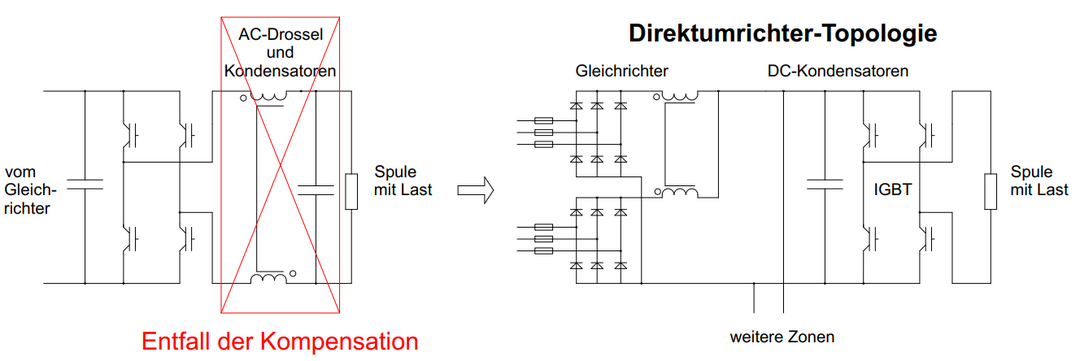
\includegraphics[width=0.85\linewidth]{images/direktumrichtergrund.png}
\end{center}

Eigenschaften:
\begin{itemize}
    \item Keine Gleichstrom-Zwischenstufe
    \item Direkte AC-AC-Wandlung
    \item Ausgangsfrequenz kleiner als Eingangsfrequenz
\end{itemize}

\crd{\textrightarrow\ Direktumrichter sind direkte AC-AC-Umrichter ohne Energiespeicher.}

% -------------------------------------------------
\subsection{Leistungsfluss und Vierquadrantenbetrieb}

\[
\boxed{P = u_2(t)\, i_2(t)}
\]

Direktumrichter erlauben:
\begin{itemize}
\item Motorbetrieb,
\item Generatorbetrieb,
\item Rückspeisung ins Netz.
\end{itemize}

Sie sind grundsätzlich vierquadrantenfähig.


\subsection{Schaltungsstruktur}

\begin{center}
    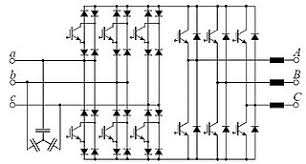
\includegraphics[width=0.85\linewidth]{images/direktumrichter_matrix.png}
\end{center}

Ein Direktumrichter besteht aus einer Matrix von bidirektionalen Schaltern,
die jede Eingangsphase mit jeder Ausgangsphase verbinden können.

Anzahl der Schalter:
\[
\cbl{3 \times 3 = 9 \text{ bidirektionale Schalter}}
\]

\subsection{Frequenzbereich}

\[
\cbl{f_2 < \frac{1}{2} f_1}
\]

Aussage:
\begin{itemize}
    \item Ausgangsfrequenz ist kleiner als Netzfrequenz
    \item Begrenzung durch Kommutierungsbedingungen
\end{itemize}

% -------------------------------------------------

\subsection{Kommutierung}

\begin{center}
    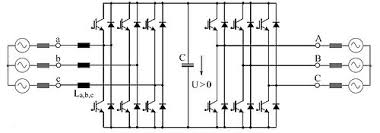
\includegraphics[width=0.85\linewidth]{images/direktumrichter_kommutierung.png}
\end{center}

Bei der Kommutierung darf \textbf{keine Netzphase kurzgeschlossen} und
\textbf{keine Lastphase unterbrochen} werden.

Grundregeln:
\begin{itemize}
    \item Niemals zwei Netzphasen kurzschliessen
    \item Niemals Laststrom unterbrechen
\end{itemize}

\crd{\textrightarrow\ Kommutierung ist das Hauptproblem des Direktumrichters.}

% -------------------------------------------------

\subsection{Eigenschaften und Einordnung}

\begin{itemize}
    \item Sehr robuste Industrieumrichter
    \item Hoher Wirkungsgrad
    \item Komplexe Steuerung
\end{itemize}

\subsection{Vergleich Direktumrichter -- Wechselrichter}

\begin{center}
\begin{tabular}{l|c|c}
 & Direktumrichter & Wechselrichter \\ \hline
Zwischenkreis & nein & \cbl{ja} \\
Eingang & AC & AC/DC \\
Ausgang & AC & AC \\
Frequenzbereich & $f_2 < \frac{1}{2}f_1$ & \cbl{frei wählbar} \\
\end{tabular}
\end{center}

\subsection{Merksätze}

\begin{itemize}
    \item Direktumrichter sind direkte AC-AC-Umrichter.
    \item Keine Zwischenkreisspannung vorhanden.
    \item Ausgangsfrequenz ist begrenzt.
\end{itemize}
